%%%%%%%%%%%%%%%%%%%%%%%%%%%%%%%%%%%%%%%%%%%%%%%%%%%%%%%%%%%%%%%%%%%%%%%%%%%%%%%%
%%%%%%%%%%%%%%%%%%   Vorlage für eine Abschlussarbeit   %%%%%%%%%%%%%%%%%%%%%%%%
%%%%%%%%%%%%%%%%%%%%%%%%%%%%%%%%%%%%%%%%%%%%%%%%%%%%%%%%%%%%%%%%%%%%%%%%%%%%%%%%

% Erstellt von Maximilian Nöthe, <maximilian.noethe@tu-dortmund.de>
% ausgelegt für lualatex und Biblatex mit biber

% Kompilieren mit
% latexmk --lualatex --output-directory=build thesis.tex
% oder einfach mit:
% make

\documentclass[
  % tucolor,       % remove for less green,
  BCOR=12mm,     % 12mm binding corrections, adjust to fit your binding
  parskip=half,  % new paragraphs start with half line vertical space
  open=any,      % chapters start on both odd and even pages
  cleardoublepage=plain,  % no header/footer on blank pages
]{tudothesis}


% Warning, if another latex run is needed
\usepackage[aux]{rerunfilecheck}

% just list chapters and sections in the toc, not subsections or smaller
\setcounter{tocdepth}{1}

%------------------------------------------------------------------------------
%------------------------------ Fonts, Unicode, Language ----------------------
%------------------------------------------------------------------------------
\usepackage{fontspec}
\defaultfontfeatures{Ligatures=TeX}  % -- becomes en-dash etc.

% load english (for abstract) and ngerman language
% the main language has to come last
\usepackage[american, ngerman]{babel}

% intelligent quotation marks, language and nesting sensitive
\usepackage[autostyle]{csquotes}

% microtypographical features, makes the text look nicer on the small scale
\usepackage{microtype}

%------------------------------------------------------------------------------
%------------------------ Math Packages and settings --------------------------
%------------------------------------------------------------------------------

\usepackage{amsmath}
\usepackage{amssymb}
\usepackage{mathtools}

% Enable Unicode-Math and follow the ISO-Standards for typesetting math
\usepackage[
  math-style=ISO,
  bold-style=ISO,
  sans-style=italic,
  nabla=upright,
  partial=upright,
]{unicode-math}
\setmathfont{Latin Modern Math}

% nice, small fracs for the text with \sfrac{}{}
\usepackage{xfrac}

\DeclarePairedDelimiter{\abs}{\lvert}{\rvert}


%------------------------------------------------------------------------------
%---------------------------- Numbers and Units -------------------------------
%------------------------------------------------------------------------------

\usepackage[
  % locale=DE,
  separate-uncertainty=true,
  per-mode=symbol-or-fraction,
  range-phrase =  \:bis\:,
]{siunitx}
\sisetup{math-micro=\text{µ},text-micro=µ}
\DeclareSIUnit[]{\langmuir}{\text{L}}
\DeclareSIUnit[]{\torr}{\text{torr}}
\DeclareSIUnit[]{\ML}{\text{ML}}
\DeclareSIUnit\angstrom{Å}
\DeclareSIUnit\bar{bar}

%------------------------------------------------------------------------------
%---------------------------- chemische Formeln -------------------------------
%------------------------------------------------------------------------------
\usepackage[
  version=4,
  math-greek=default,
  text-greek=default,
] {mhchem}

%------------------------------------------------------------------------------
%-------------------------------- tables  -------------------------------------
%------------------------------------------------------------------------------

\usepackage{booktabs}       % \toprule, \midrule, \bottomrule, etc

%------------------------------------------------------------------------------
%-------------------------------- graphics -------------------------------------
%------------------------------------------------------------------------------

\usepackage{graphicx}
\graphicspath{{./content/pictures}}
% currently broken
% \usepackage{grffile}

% allow figures to be placed in the running text by default:
\usepackage{scrhack}
\usepackage{float}
\usepackage[width=0.9\textwidth]{subcaption}
% \usepackage{sidecap} % makes Caption and figure byside
% \usepackage{wrapfig} %für text umflossene Bilder, funktioniert aber nicht so
% \floatplacement{figure}{htbp}
% \floatplacement{SCfigure}{htbp} % makes Caption and figure byside
% \sidecaptionvpos{figure}{c} % set if the sidecaption is centered to image
% \floatplacement{table}{htbp}


% keep figures and tables in the section
\usepackage[section, below]{placeins}


%------------------------------------------------------------------------------
%---------------------- customize list environments ---------------------------
%------------------------------------------------------------------------------

\usepackage{enumitem}
\usepackage{pdfpages} % to include the Eidesstaatliche Versicherung

%------------------------------------------------------------------------------
%------------------------------ Bibliographie ---------------------------------
%------------------------------------------------------------------------------

\usepackage[
  backend=biber,   % use modern biber backend
  autolang=hyphen, % load hyphenation rules for if language of bibentry is not
                   % german, has to be loaded with \setotherlanguages
                   % in the references.bib use langid={en} for english sources
  sorting=none,
  % firstinits=true,
]{biblatex}
\addbibresource{references.bib}  % the bib file to use
\DefineBibliographyStrings{german}{andothers = {{et\,al\adddot}}}  % replace u.a. with et al.


% Last packages, do not change order or insert new packages after these ones
\usepackage[pdfusetitle, unicode, linkbordercolor=tugreen, citebordercolor=tugreen]{hyperref}
\usepackage{bookmark}
\usepackage[shortcuts]{extdash}

%------------------------------------------------------------------------------
%-------------------------    Angaben zur Arbeit   ----------------------------
%------------------------------------------------------------------------------

\author{Valentin Mischke}
\title{Organische Moleküle auf Antiferromagneten: Eine Photoemissionsstudie}
\date{2021}
\birthplace{Haan}
\chair{Lehrstuhl für Experimentelle Physik VI}
\division{Fakultät Physik}
\thesisclass{Master of Science}
\submissiondate{02. Dezember 2021}
\firstcorrector{Prof.~Dr.~Mirko Cinchetti}
\secondcorrector{Prof.~Dr.~Heinz Hövel}
% \secondsupervisor{M.~Sc.~David Janas}
\supervisor{Dr.~Giovanni Zamborlini}

% tu logo on top of the titlepage
\titlehead{\includegraphics[height=1.5cm]{logos/tu-logo.pdf}}

\begin{document}
\frontmatter
\maketitle

% Gutachterseite
\makecorrectorpage

% hier beginnt der Vorspann, nummeriert in römischen Zahlen
\thispagestyle{plain}

\section*{Kurzfassung}


\section*{Abstract}
\begin{foreignlanguage}{english}

\end{foreignlanguage}

\tableofcontents

\mainmatter
% Hier beginnt der Inhalt mit Seite 1 in arabischen Ziffern
\chapter{Einleitung}
    % Wieso
    Die Anzahl an Menschen, die digitale Geräte wie etwa ein Smartphone nutzen, steigt stetig~\cite{Statista}.
    Damit steigt auch der Energie- und Materialbedarf der Digitalisierung an.
    Steigerung gibt es aktuell kaum noch in der Effizenz, Bauteilgröße und Minimierung der Leistungsaufnahme.
    Wie schon der Nobelpreisträger H. Kroemer im Jahre 2000 sagte, ist die Grenzfläche das Bauteil (\textit{"The interface is the device"}).
    Im Gegensatz zur herkömmlich Halbleiterbasierten Technik stehen neue Materialkombinationen aus organischen und anorganischen Materialien.
    Durch ihre Anwendung in organischen Halbleitertechnik wie den OLEDs (\textit{organic light emitting diodes}) und OFETs (\textit{organic field effect transistors}) ergibt sich ein großes Intresse auf diesem Gebiet in den letzten Jahren~\cite{Uni-Tübingen}.
    So könnten Moleküle z.B. optisch angeregt werden und damit Spinwellen im Antiferromagneten auslösen. 
    An anderer Stelle werden diese Spinwellen von einem weiteren Molekül aufgenommen und in ein einfach messbares Signal umgewandelt~\cite{SINFONIA}.
    Da die Frequenzen von Spinwellen in Antiferromagneten im \si{\tera\hertz}-Bereich liegen, kann dadurch die Taktung elektronischer Geräte im Vergleich zur heutigen Zeit noch einmal deutlich erhöht werden~\cite{AFM_5}.
    Bei diesem Prozess entfällt die Joulsche Wärme, da Spinwellen kein Transport von Elektronen, wie bei herkömlichen auf Halbleiter basierenden Komponenten stattfindet~\cite{AFM_3}.
    Folglich muss für die selben Prozesse eine geringere Energie aufgewendet werden.
   
    % Grenzfläche
    Die Verwendung von Grenzflächen von organisch-anorganischen Materialien ist viel Versprechend aufgrund der großen Vielzahl an zur Verfügung stehenden Materialien.
    So sind die Eigenschaften von organischen Materialien auf Oberflächen mit dessen Eigenschaften eng verknüpft.
    Zusätzlich sorgt die räumliche Einschränkung zu weiteren Zuständen und Oberflächeneffekte sind stark ausgeprägt.
    Die Erforschung der elektronischen und magnetischen Eigenschaften und deren Kombination dieser Schichtsysteme stehen im Fokus vieler Forschungsprojekte.
    Ziel ist es eine externe Eingabe umzuwandeln und an das Substrat weiter zu geben um dies dann nutzbar zu machen.
    Dies über magnetische Eigenschaften zu realisieren, bietet den Vorteil, dass keine Ladung transportiert werden muss und somit die Geschwindigkeit erhöht werden kann.
    Hierzu soll mittels optischer Stimulation oder einem äußeren Felde die chemische und physikalische Eigenschaft des Moleküls beeinflusst werden.
    Aufgrund der Verknüpfung mit den Eigenschaften der Grenzfläche können diese hier weiter transportiert oder umgewandelt werden~\cite{IF_16}.
    Der Energieaufwand für Anregungen in den oranischen Materialien ist geringer als in den anorganischen Materialien und kann somit einfacher realisiert werden.
    Es hat sich gezeigt, dass sich die magnetischen Eigenschaften der Molekül wie auch der Grenzfläche durch die entsprechende Wahl und Schichtdicke, die mit der Hybridisierung einher gehen, beeinflussen lassen~\cite{IF_16}.
    Dabei hat sich besonders der Prozess der Chemisorption als tragender Beitrag erwiesen.

    % Moleküle
    Die große Anpassbarkeit von organischen Molekülen im Bezug auf ihre Struktur und Zusammensetzung sind viel Versprechend.
    Einher gehen damit ihre elektronischen Eigenschaften, die somit für den jeweiligen Prozess optimiert werden können~\cite{scholl_chapter_2018}.
    Auch die geringe Größe der Moleküle ermöglicht eine weiter Minimierung der elektronischen Komponenten.
    Die Verwendung von Molekülen, die aus leichten Atomen bestehen, reduziert des Weiteren auch das Gewicht der entsprechenden Bauteile, was besonders für mobile Geräte interessant ist.
    Durch den verzicht auf giftige Schwermetalle und andere Substanzen sind solche organischen Materialien umweltfreundlicher als ihre Konkurenten der heutigen Technik~\cite{scholl_chapter_2018}.
    Auch der immer größere Bedarf und damit steigende Preise und Engpässe an Halbleitern sorgen für die Nachfrage nach Alternativen~\cite{Idealo}.

    % AFM+TMOs
    Bisher standen vermehrt ferromagnetisch-organische Grenzflächen bei der Forschung nach Spin-elektronischen Bauteilen im Fokus~\cite{ma-DJ}.
    Um die Vorteile der antiferromagnetischen Materialien, der Anpassbarkeit vom Kontaktwiderstand und Struktur zu erhalten sind Übergangsmetalloxide ideale Kandidaten.
    Ihre elektronischen Eigenschaften, insbesondere ihre Austrittsarbeit, lassen sich einfach modifizieren.
    Dies betrifft besonders die Energiedifferenz zwischen Fermi und HOMO beziehungsweise LUMO, welche ein entscheidener Schlüssel für die Anwendung darstellt~\cite{5A_4}.
    Heutzutage werden Übergangsmetalloxide bereits eingesetzt um als Zwischenschichten zwischen Elektrode und organischer Schicht in oragnischen Bauteilen den Kontaktwiderstand zu reduzieren und die Energieniveauanpassung der Moleküle zu ermöglichen~\cite{IF_11}.
    Die Verwendung von antiferromagnetischen Übergangsmetalloxiden zeigt eine größere Stabilität hinsichtlich ihrer Magnetisierung und schneller Dynamiken als es für Ferromagneten bekannt ist~\cite{AFM_1}.
    Durch die Reduktion in iherer Größe lassen sich die magnetischen Momente der Ferromagneten schwieriger Ausrichten als bei Antiferromagneten.
    Hinzukommend können isolierende Antiferromagneten einen elektronischen Spin-Strom in einen magnonischen Spin-Strom umwandeln~\cite{AFM_1}.
    Durch die Verwendung von Magnonen entfällt die Stromversorgung.
    Hierdurch wird zum einen Energie gespart zum anderen fällt ein Problem bei der Chipproduktion, der Spannungsversorgungsleitungen inerhalb des Chips, weg~\cite{AFM_3}.
    Auch die Frequenz der Magnonen ist größer als bei ihren Konkurrenten der ferromagnetischen Übergangsmetalloxide~\cite{AFM_5}.
    Heutzutage finden Antiferromagneten als eigene interaktive Lage bei kleineren Leseköpfen von Festplatten Anwendung, welche auf dem Riesenmagnetowiderstand (GMR, \textit{giant magnetoresistance}) beruhen.
    Sie dienen nicht mehr nur als Fixierungslage für eine ferromagnetische Schicht sondern eigenständig in Kombination mit Molekülen und einer ferromagnetischen Lage~\cite{bagrets_single_2012}.

    % Ansatz und Systeme
    Erste theoretische Berechnungen zeigen bei der Kombination von Molekülen und Antiferromagneten lokale Spinpolarisationen, welche die Kerneigenschaft von Spinterfaces darstellt~\cite{AFM_2}.
    Mit dem Ansatz der Kopplung von Antiferromagneten und Molekülen beschäftigt sich das europäischen Forschungsprojekt Sinfonia~\cite{SINFONIA}.
    Hierbei sollen sich die Moleküle auf einer antiferromagnetischen Oberfläche regelmäßig anordnen, um diese dann gezielt zu manipulieren.
    Ferner sollen diese genutzt werden um Spinwellen, so genannte Magnonen zu generieren und zu detektieren.

    Für das Verständnis über die ablaufenden Prozesse, wie die Molekül-Substrat-Wechselwirkung an der Grenzfläche sind die Informationen über die elektronische Struktur unabdingbar.
    Um solche selbstanordnenden Moleküle hinsichtlich ihrer elektronischen Struktur zu untersuchen ist die Verwendung der Photoemissionorbitaltomographie eine starke Methode.
    % Um solche selbstanordnenden Moleküle hinsichtlich ihrer elektronischen Struktur zu untersuchen ist die Verwendung der Photoemissionorbitaltomographie, impulsaufgelösten Photoemissionsmessungen mit ab initio Berechnungen mit Hilfe der Dichtefunktionaltheorie durchführt, welche eine starke Methode.
    Sie liefert die eindeutige Identifizierung der beteiligten Molekülorbitale und deren azimuntalen Ausrichtung~\cite{MM_2, MM_5}.
    
    Das Aufbringen der Moleküle auf ein antiferromagnetisches Substrat, wie dem Eisenmonooxid ist interessant, da Eisen ein häufig eingesetztes Material ist und in einer großen Anzahl zur Verfügung steht. % kann zu neuen Phänomenen und Eigenschaften führen.
    Die Erweiterung auf die Kombination mit einer polaren und somit reaktiven antiferromagnetischen Oberfläche wie die \ce{NiO} (111)-Oberfläche stellt eine neue Idee dar~\cite{cappus_hydroxyl_1993}.
    Auf dieser Oberfläche sind alle Spins in die selbe Richtung ausgerichtet, was einen imensen Vorteil bei der Maipulation bieten könnte.
    Das untersuchte Pentacene wird heute schon in einigen organisch elektronischen Bauteilen eingesetzt~\cite{5A_4}.
    In Folge dessen werden in dieser Arbeit erste Charakterisierungen für potenzielle Substrate und Moleküle untersucht.

    % Um die Art der Interaktion zu bestimmen um die Performance zu verbessern eignet sich die Molekülorbitaltomographie besonders gut.
    % Dieses System kann also hinsichtlich dem großen Energiebedarf zur Kühlung in Rechenzentern diesen senken.
    % Aktuelle Entwicklungen der Halbleiterindustrie auf CMOS Basis sind komm noch in ihrer Größe minimierbar, auch hier könnte das System zu einer kleineren Bauweise beitragen. 
    % Somit wären gleich mehrer Probleme der IT-Industrie gleichzeitig gelöst.
    % 
    % NiO zeigt bereits Eigenschaften des Katalisators~\cite{kunz_chemisorption_1985}, eine Erweiterung und Verbesserung mit Hilfe der Moleküle wäre denkbar.
\begin{itemize}
    \item the ferromagnetic/organic interface of organic based spintronic devices has been target of research because evidence was found for its excessive impact on the overall device performances [15, 16, 17]. (DJ)
    \item PEN in OFETS (\url{https://www.sciencedirect.com/science/article/abs/pii/S0065272518300357})
\end{itemize}


\chapter{Grundlagen}
    In diesem Kapitel wird eine Einführung in die Grundlegenden Eigenschaften der untersuchten Systeme gegeben.
    Zunächst geht es um die Oberflächen von Festkörpern, da dies in der vorliegenden Arbeit genauer untersucht werden.
    Anschließend geht es um den Antiferromagnetismus, welcher die magnetischen Strukturen innerhalb der Proben beschreibt.
    Dann geht es um die Wechselwirkung zwischen Oberflächen und le und wie diese sich auf der Oberfläche bezüglich ihrer geometrischen und elektronischen Struktur verändern.
    Zuletzt werden dann die Oberflächen und Moleküle eingeführt, welche zur Präperation der verwendeten Proben genutzt wurden.

    \section{Übergangsmetalloxide}
        Übergangsmetalloxide finden sich in einer Vielzahl in unserer Umwelt, meist jedoch unter anderem Namen.
        So ist der Rost wohl eins der bekanntesten, dabei handelt es sich um eine Form des Eisenoxids.
        Magnetit hingegen ist in der Wissenschaft sehr bekannt, da es zu den ersten entdecken magnetischen Materialien gehört.
        Übergangsmetalloxide haben in den letzten Jahren in der Wissenschaft immer mehr Aufmerksamkeit auf sich gezogen.
        Grund dafür ist ihre straken Elektron-Elektron-Wechselwirkung, sowie dessen einfachen Herstellung.
        Durch die Reduktion auf dünne Filme und damit verbundenen Einschränkung ergeben sich neue spannende Eigenschaften.

        Viele der Übergangsmetalloxide zeigen Ferro- oder Antiferromagnetismus. 
        Auch ihre chemischen und elektrochemischen Eigenschaften lassen sie sich durch unterschiedliche Präperationsprozesse perfekt anpassen\cite{Uni-Tübingen}.
        So werden sie häufig zur Kathalyse eingestezt oder als Halbleiter.

        Übergangsmetalloxide bestehen dabei aus einem Übergangsmetall, dem Kation und als Anion kommen Sauerstoffatome zum Einsatz.
        Die kristallienen Eigenschaften der Übergangsmetalloxide sind schon weit erforscht, dabei fehlt es aber an Forschung zur Oberfläche und dünnen Filmen.
        Aus diesem Grund und der großen Vielzahl stehen Übergangsmetalloxide im Fokus der aktuellen Forschung.
        Dabei spielen die Polarität, Anzahl ungesättigter Bindungen wie auch Defekte eine entscheidene Rolle in der Oberflächenrekonstruktion.
        Die hier untersuchten Monooxide Systeme mit der Beteiligung von 3d-Übergangsmetallen kristallisieren in der Kochsalzstruktur (\ce{NiO}, \ce{FeO})
        Im Gegensatz dazu kristallisiert das \ce{Fe3O4} in der inversen Spinellstruktur.

        Die Oberflächen der Kochsalzstruktur mit der (100)-Orientierung sind meist stabil, wohingegen die der (111)-Orientierung instabil sind.
        Dies liegt an der polaren Oberfläche der (111)-Orientierung un des damit verbundenen großen Oberflächendipolmoments. 
        Anzumerken bleibt, dass dabei die Sauerstoff terminierte Oberfläche stabiler als die metallisch terminierte Oberfläche ist.
        Ursache ist die einfachere Polarisation des Sauerstffatoms, was das Oberflächendipolmoment reduzieren kann \cite{al-abadleh_oxide_2003}.

        Bei der Betrachtung der Bandstruktur der Übergangsmetalloxide ist zu beachten, dass diese eine Bandlücke zwischen Valenz- und Leitungsband aufweisen.
        Diese Bandlücke liegt dabei zwischen den besetzen Sauerstoffzuständen und den unbesetzten d-Zuständen des Übergangsmetall.
        Denn durch die Hybridisierung zwischen den p-Orbitalen des Sauerstoffs und den s-Orbital des Übergangsmetall fallen diese als Abschirmung bei den d-Orbitalen weg.
        Diese spalten sich dadurch auf und entsteht die Bandlücke.
        Beachtung erhalten da besonders also die stark korrelierten und stark delokalierten Elektronen der d-Orbitale.
        Dabei gibt es zwei Arte

        Wird die Wechselwirkung in der Kombination aus Übergangsmetall und Sauerstoff beachtet, dass die 

        Die Bandstruktur des Kristalls wird im Valenzbandbereich durch die überlappenden 2p Orbitale des Sauerstoffs im niederenergetischen Bereich dominiert.
        Zu höheren Energien hin rührt die Bandstruktur von den überlappenden d Orbitalen der Übergangsmetalle her.
        Dabei sind die 2p Zustände strak bestezt wohingegen die d Zustände nur schwach besetzt sind.
        Der Übergang zum Leitungsband weist dabei eine Bandlücke auf, es handelt sich also im Halbleiter oder Isolatoren.

        Vor allem in dem \ce{Fe3O4} in dem das Eisen als (2+) und (3+) Ion vorkommt auf unterschiedlichen Gitterplätzen (tetraedisch oder oktaedrisch) kommt es zu unterschiedlichen Aufspaltungen der $e_g$ und $t_{2g}$ Energieniveaus.

        \begin{itemize}
            \item s Orbitale spärisch symmmetrisch
            \item \textbf{https://www.youtube.com/watch?v=gWXoGP6DbM8}
            \item p Orbitale hantelförmig (3 Stück)
            \item d Orbitale (2 eg und 3 tsg -> fünf stück) Verschiedene Symmetrien
            \item WW zwischen Ladung, Orbitale Gitter und Spin -> Magnetismus
            \item Oberflächen und Grenzflächen zeigen neue Eigenschaften und Phasen -> Anwendung 
            \item "The interface is the device" von H. Kroemer (Nobelpreis Physik 2000)
            \item Symmetriebrechung, Verspannung (WW mit Substrat), Polarität, Filmdicke, Kristallograpische Orienteierung
        \end{itemize}

        Die untersuchten Übergangsmetalle gehören beide zu den 3d Übergangsmetallen.

        
        \begin{itemize}
            \item \textbf{Däne - 2008 - Beschreibung der elektronischen Struktur korrelier.pdf}
            \item 3d-Übergangsmetalloxide sind Isolatoren (Mott-Hubbard oder Charge Transfer)
            \item In Übergangsmetallen Coulomb Abstoßung der d elektronen durch delokalierte s abgeschirmt d Bänder folglich aufgespalpten
            \item In dessen Oxiden nur hybridisieren diese s mit dem p des O und sind gebunden -> Aufspaltung in p und s artige Zustände, s unbesetzten
            \item Es kommt zur größeren Aufspaltung der d in M und damit der Bandlücke
            \item zusätzlich energie zwischen platzwechsel O-M kleiner als M-M (Coulomb)
            \item Bandlücke zwischen dem O-Zustand und unbestzte d Zustand
        \end{itemize}

        Im späteren Verlauf wird genauer auf die untersuchten Übergangsmetalloxide eingegangen.

    
    \section{Antiferromagneten}
        Antiferromagneten (AFM) zeichnen sich dadurch aus, dass Sie nach außen hin kein permanetes magnetisches Moment aufweisen.
        Vereinfacht sind im Inneren die magnetischen Momente vom gleichen Betrag und nebeneinander liegende Momente sind antiparallel unterinander ausgerichtet \cite{Suter}.
        Dieser Zustand ist allerdings nur unterhalb der Néel-Temperatur $T_\text{N}$ stabil, oberhalb verhälten sich die Antiferromagneten paramagnetisch.
        Um das Phänomen des Antiferromagnetismus zu erklären bedarf der quantenmechanischen Erklärung unter Beachtung des Pauli Verbots und der Hundschen Regeln \cite{TUChemnitz}.
        Es ergibt sich der Austauschwechselwirkungshamiltonien $H_\text{A} = - J_{ik} \vec{S_i}\cdot\vec{S_k}$ der die direkte Wechselwirkung der Spins berücksichtigt.
        Für $J_{ik} < 0$ ergibt sich die antiferromagnetische Kopplung und für $J_{ik} > 0$ eine ferromagnetische Kopplung.
        $J_{ik}$ spiegelt dabei die Stärke der Austauschwechselwirkung wieder und folgt aus dem Überlapp der Wellenfunktionen der beteiligten Elektronen.
        Um eine Aussage über die Ordnung im Antiferromagnet zutreffen gibt es den Ordnungsparameter $L = S^{\uparrow} - S^{\downarrow}$.
        Hierbei ist $S^{\uparrow}$ beziehungsweise $S^{\downarrow}$ der Spin der Untergitter.

        \begin{itemize}
            \item fcc Gitter (111) und (100) Oberfläche
            \item real und reziproker Raum
            \item Bandstruktur
            \item Oberflächenzustände?
        \end{itemize}

        % \subsection{Superaustausch}
        % \label{sec:Super}
        \begin{figure}
            \centering
            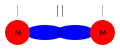
\includegraphics[width=0.6\textwidth]{AFM2.pdf}
            \caption{Darstellung zur Veranschaulichung der antiferromagnetischen Kopplung.
            Als Ligand fungiert hier ein Sauerstoffatom mit seinem p-Orbital (blau).
            Die Spins der d-Orbitale der Metalle (rot) koppeln ferromagnetische mit denen des Sauerstoffs.
            So entsteht die antiferromagnetische Kopplung der beiden Metallatome.}
            \label{fig:AFM}
        \end{figure}
        Ursache des Antiferromagnetismus ist der Superaustausch.
        Beim Superaustausch koppeln zwei Atome mit einem magnetischen Moment über ein weiteres nicht magnetische Atom. 
        Dabei kann die Kopplung ferro- oder antiferromagnetisch sein, meist jedoch antiferromagnetisch \cite{AFM_1}.
        Sind die beiden koppelnden magnetischen Momente nicht gleich groß, so tritt Ferrimagnetismus auf, es gibt dann eine makroskopische Magnetisierung.
        Der Superaustausch ist winkelabhängig, da es dabei um den Überlapp der Orbitale geht.
        Für die Erklärung wird sich hier nur auf die \SI{180}{\degree} Wechselwirkung beschränkt.
        Beispielhaft ist die Kopplung in \autoref{fig:AFM} dargestellt.
        Es kommt bei diesem indirekten Austausch nicht zu einem Überlapp der spintragenden Wellenfunktionen sondern zu der Vermittlung der langreichweitigen Ordnung über einen Liganden.
        Direkter Austausch sorgt für ferromagnetische Kopplung benachbarter andersartige (nicht magnetische) Atome.
        Zwischen Metall und Ligand herscht also direkte Austauschwechselwirkung und damit eine indirekte Austauschwechselwirkung, der Superaustausch zum übernächsten Atom, einem weiteren Metallatom.
        Bei den vorliegenden Metalloxiden ist es so, dass die Elektronen der Metallatom des nicht vollen 3d Oribtals über die 2p Orbitale des Sauerstoffs koppeln.
        Da dieses Orbital voll ist, müssen die Elektronen unterschiedliche Spinrichtung haben.
        Damit besitzten die Sauerstoffatome auch kein eigenes magnetisches Moment.
        Somit ist dann die Wechselwirkung über das Sauerstoffatom hinweg dann antiferromagnetisch.
        Es ergeben sich so zwei Untergitter, welche unterschiedlicher Spinrichtung sind, die Gesamtmagnetisierung ist also wie für Antiferromagneten erwartet Null.
        % Die Wellenfunktionen der Kationen überlappen nur gering und da die Austauschwechselwirkung nur geringe Reichweiten hat können nur die 3d und 2p überlappen.
        % \begin{itemize}
        %     \item Magnonen
        % \end{itemize}
        
        Die Anwenungen des Antiferromagnetismus ist zum Beispiel der nutzen als \textit{Pinning}-Lage, die in spinelektronischen Bauteilen die Orientierung einer ferromagnetischen Schicht festlegt.
        
            
    
    \section{Wechselwirkung von Oberfläche mit Molekülen}
        Moleküle haben im Gegensatz zu Festkörpern, energetisch separierte Zustände, die Orbitale.
        Werden Molekül auf eine Oberfläche aufgebracht so kommt es zur Wechselwirkung zwischen diesen und der Struktur der Oberfläche.
        Bei der Wechselwirkung von Molekülen mit Oberflächen wird in zwei Arten der Adsorption unterschieden. 
        Zum Einen der Physisorption und der Chemisorption, welche wiederum in stark und schwach unterschieden wird.
        Zwischen den beiden Adsorptionsarten lässt sich durch ihre Bindungsstärke von den Molekülen auf dem Substrat unterscheiden.
        Dabei wird als Bindungsstärke die Energie bezeichnet, die nötig ist um ein Molekül von der Oberfläche zu lösen.
        In beiden Fällen handelt es sich um eine Adsorption die auch die Oberflächenstruktur des Substrates beeinflussen können.
        So können neue Zustände entstehen und vorhandene Eigenschaften stark verändert werden.
        %~\cite{ma-DJ
        
        \subsection{Physisorption}
            Bei der Physisorption spielt maßgeblich die Van-der-Waals-Kraft eine Rolle, hat also eine eher geringe Bindungsenergie der Moleküle zum Substrat~\cite{cinchetti_activating_2017}.
            Charakteristisch für die Physisorption ist die Abwesenheit von chemischen Bindungen sowie einen Substrat-Adsorbat-Abstand von mehr als \SI{3}{\angstrom}. %~\cite{bergenti_spinterface_2019}
            Da die Wechselwirkung bei der Physisorption nur gering ist werden die Eigenschaften der Oberfläche und des Moleküles nur schwach beeinflusst~\cite{bergenti_spinterface_2019}.
            Allerdings kann es beim Substrat zu Relaxation kommen.
            Die Bindungen des Moleküls werden nur schwach beeinflusst, sodass sie den Eigenschaften aus der Gasphase stark ähneln~\cite{cinchetti_activating_2017}.
            Die Van-der-Waals-Kraft gehört zu den elektrostatischen Kräften, es werden also keine Elektronen mit dem Substrat ausgetauscht~\cite{bergenti_spinterface_2019}.
            Allein die Induzierung und Fluktuation von Dipolen führt zu dieser Bindung zwischen Molekül und Substrat.
            Die Van-der-Waals-Kraft kann man in drei Arten unterteilen:
            \begin{itemize}
                \item \textbf{Dipol-Dipol-Kraft:} Sie ist die Kraft zwischen zwei permanenten Dipolen, die Keeson-Wechselwirkung.
                \item \textbf{Dipol-induzierter-Dipol-Kraft:} Die Wechselwirkung zwischen einem induziertem Dipol und einem Dipol wird auch als Debye-Wechselwirkung bezeichnet.
                \item \textbf{Londonsche Dispersions-Wechselwirkung:} Zwischen zwei induzierten Dipolen wirkt die Londonsche Dispersions-Wechselwirkung, sie dominiert meist die Van-der-Waals Kraft.
            \end{itemize}

            Die Physisorption kann durch zwei Potetiale beschrieben werden.
            Das eine Potential wirkt repulsiv und resultiert aus dem Pauliverbot.
            Kommen sich Molekülorbital und Substratorbital zunah, überlappen diese.
            Auf Grund des Pauliverbots dürfen keine zwei Elektronen dann in allen Quantenzahlen übereinstimmen und es resultiert in eine abstoßende Kraft.
            Attraktives Potentential resultiert dabei aus der Debye-Wechselwirkung.
            So kommt es beim Gleichgewicht zu einem stabilen Substrat-Molekül-Abstand.
            Das gesamtpotential ist auch als Lennard-Jones-Potential bekannt.
            Vermehrt tritt die Physisorption bei Halbleitern und Isolatoren auf, da die Molekülzustände in der Bandlücke liegen und so keine Bindung mit dem Substrat eigegangen werden kann~\cite{IF_1}.
        
        \subsection{Chemisorption}
            % Im Gegensatz zur Physisorption findet bei der Chemisorption  ein Austausch von Elektronen stattfinden.
            Im Gegensatz zur Physisorption sind die Bindungen um Einiges stärker und führen somit zu Veränderung am Substrat wie auch den Molekülen~\cite{bergenti_spinterface_2019}.
            Ferner wird von Chemisorption gesprochen, wenn die Stärke der Wechselwirkung größer als \SI{1}{\electronvolt} ist~\cite{muscat_chemisorption_1978}.
            Aber dies allein ist nicht ausschlaggebend, es muss eine chemische Veränderung auftreten.
            Dabei kann es sich um kovalente und ionische Bindungen handeln und es kann zum Ladungsaustausch und/oder Hybridisierung kommen~\cite{harutyunyan_hybridisation_2013}.
            Beim Ladungsaustausch kann ein zunächst unbesetztes Orbital unter die Fermikante rutschen und besetzt werden, es kann also neben den strukturellen auch zu elektronischen Veränderungen kommen.
            Im Gegensatz dazu können bei der Hybridisierung mehrer Zustände vom Molekül und/oder Oberfläche durchmischt werden.
            Verbreiterungen, Verschiebungen und auch Aufspaltungen von Molekülzuständen kann die Folge sein~\cite{IF_1}.

            \begin{figure}
                \centering
                \includegraphics[width=0.6\textwidth]{Chemisorption2.PNG}
                \caption{Das adsorbierte Molekül hybridiziert mit dem s-/p-Band des Substartes (1), der schwachen Chemisorption.
                In einem weiteren Schritt kommt es dann zur starken Chemisorption durch Einbindung der d-Bänder (2, oben), es entsteht ein bindendes und ein antibindenes Orbital.
                Durch die Lage der d-Bänder werden nun das bindenden und antibindendene Orbital besetzt, dadurch kommt es zu einer repulsiven Kraft und die Bindung wird wieder geschwächt (unten). Aus~\cite{IF_1}.}
                \label{fig:Chemisorption}
            \end{figure}
            Schwache Bindungen werden meist durch die Wechselwirkung mit den breiten s- oder p-Bändern hervorgerufen.
            Wodurch sich das Energieniveau der Moleküle absenkt und verbreitert, siehe dazu in \autoref{fig:Chemisorption}.
            Für die starke Chemisorption folgt ein weiterer Schritt, der nun abgesenkte Zustand überlappt mit dem der näherungsweise d-Bänder.
            Es bilden sich bindende und antibindendene Zustände aus.
            Ja nach Lage des Ferminiveaus wird nur der bindenden Zustand (starke Adsorption) oder auch (nur teilweise) der antibindene Zustand gefüllt, wodurch repulsiv Kräfte auftreten.
            Ferner beeinflusst auch die Ausdehnung der d-Bänder die Stärke der Chemisorption.
        
        \subsection{Selbstanordnung}
            \begin{figure}
                \centering
                \includegraphics[width=0.6\textwidth]{Adsorbate}
                \caption{Die Adsorbateplätze für verschieden orientierte Oberflächen eines flächenzentrierten Kristalls.
                Es gibt Plätze direkt oberhalb eines Substratatoms (\textit{on top} - t).
                Zwischen zwei Substratatomen gibt es kurze (b) und lange (b') Brückenplätze (\textit{bridge}), sowie Muldenplätze hexagonaler dicht gepacktester Struktur (\textit{hollow} - h) und flächenzentrierter Struktur (h'). Aus~\cite{Fauster}.}
                \label{fig:Adsorbate}
            \end{figure}
            Einige Moleküle ordnen sich regelmäßig auf dem Substrat an, dieser Effekt wird Selbstanordnung genannt.
            Dabei bilden die Moleküle eine Überstruktur im Vergleich zum Gitter des Substrates.
            Gewünscht ist dies, da dann die Molekül einheitlich auf der Oberfläche orientiert sind und somit auch ihre Orbitale, dies ist notwendig für die Molekülorbital-Tomographie (s. \autoref{sec:MOT}).
            Ferner lassen sich gitteratig verteilte Moleküle gezielter manipulieren, wie es für Anwendungen notwendig ist.
            
            Moleküle stellen eine Art der Adsorbate da und können sich an verschiedene Stellen des Substrates setzen.
            Hier wird auf drei unterschiedeliche Möglichkeiten unterschieden dem Platz direkt über einem Substratatom (\textit{on top}), zwischen zwei Substratatomen (\textit{bridge}) oder in der Mitte von mehreren Substratatomen in einer Mulde (\textit{hollow}).
            Beispielhaft ist dies für einen flächenzentrierten Kristall mit verschiedenen Oberfläche in \autoref{fig:Adsorbate} dargstellt.
            Die physikalische Ursache ist noch nicht ganz klar, warum sich manche Moleküle auf einigen Substraten ordnen und andere hingegen nicht.
            Naheliegend ist, dass es mit der Wechselwirkung zusammenhängt und der Affinität Elektronen auszutauschen.
            Dies wurde bereits auf die Austrittsarbeit für einige Metaloxide hinweg untersucht \cite{greiner_universal_2012}.

            Das Wechselspiel zwischen der Molekül-Molekül-Wechselwirkung und Molekül-Substrat-Wechselwirkung definiert die finale Struktur \cite{IF_1}.
            Dabei sind vor Allem gerichtete Kräfte wichtig um die Regelmäßigkeit zu erhalten.
            Schwächste und ungerichteste Kraft ist die Van-der-Waals-Kraft, genauer die Debye-Wechselwirkung (\SIrange{0.02}{0.1}{\electronvolt}), die allerdings sehr langreichweitig ist.
            Weitere Ursache ist der Einfluss des Substrates auf die Wechselwirkung den Molekülen untereinander, z.B. durch Oszillationen des Oberflächenpotentials.
            Die Keeson-Wechselwirkung als Ursache der Dipol-Dipol-Interaktion hat ebenfalls Beteiligung an der Anordnung der Moleküle, allerdings nur wenn die Moleküle ein permanetes Dipolmoment haben.
            Mit der Wasserstoff-Brücken-Bindung (\SIrange{0.01}{1.73}{\electronvolt}) unter den Molekülen bindet sich ein Wasserstoffatom an ein elektronegativeres Atom, hierdurch kommt es zu Ladungsverschiebung innerhalb der Bindung.
            Das positivere Wasserstoffatom kann nunmehr eine elektrostatische Bindung zu einem weiteren Atom einnehmen.
            Wasserstoff-Brücken-Bindungen sind je stärker sie werden eher geradlinig gerichtete Bindungen mit einer kurzen Bindungslänge.
            Metallisch Koordination ist eine weiter Form der Bindung (\SIrange{0.5}{2}{\electronvolt}), die Moleküle funkieren als Linker zwischen einzelenen Metallatomen.
            Die stärkste und gerichteste Kraft ist jedoch die kovalente Bindung, welche gleichzeitig auch die elektronische Struktur stark beeinflusst.
            Sie ist sogar so stark, dass sie teilweise eine perfekte Selbstanordnung behindert und damit eher zu weniger geordneten Strukturen führen kann \cite{IF_1}.

            Neuste Studien zeigen, dass die Energieniveauanpassung maßgeblich durch die Austrittsarbeit beeinflusst wird \cite{IF_3}.
            Hierzu wurden verschiedene Metaloxide untersucht mit dem Ergebnis, ...

        \subsection{Energieniveau-Anpassung}
            Für die Anwendung besonders bedeutsam ist die Energieniveau-Anpassung, welche Einfluss auf den Elektronen- und Lochtransport hat~\cite{IF_4}.
            Bei Metalloxiden verschiebt sich durch die Austrittsarbeit die relative Position des Valenz- und Leitungsbandes zum Vakuumniveau \cite{IF_3}.
            Die meisten der Metalloxide haben keine besetzten Zustände nahe der Fermikante, da diese in eine Bandlücke fällt.
            Folglich ist auch Ladungsübertrag vom Substrat auf die Moleküle nur vom Valenz- oder Leitungsband aus möglich.
            Auch wenn einige Oxide Ladungsaustausch zwischen Valenzband und dem höcsten bestzten Molekülorbital (HOMO, \textit{highest occoupied molecular orbital}) zulassen so  gibt es noch kein Model, dass dies beschreibt.
            Verbreitet ist jedoch der Ansatz der Ferminiveau-Anheftung für nicht reaktive Grenzflächen zwischen Molekülen und Oxiden.

            Greiner u.a. \cite{IF_3} fanden heraus, dass die Bandstruktur des Substartes dabei nur eine untergeordnete Rolle spielt.
            Ausschlaggebend für die Energieniveau-Anpassung ist das elektrochemische Potential des Substrates mit dem Reduktionspotentials des Moleküls.
            Genauer die Differenz zwischen der Austrittsarbeit des Substrates und der Ionisationsenergie.
            Als Ionisationsenergie wird die Energie zwischen höchsten besetztem Molekülorbital und dem Vakuumlevel verstanden.
            Die Elektronenaffinität entspricht der Energie zwischen dem Vakuumlevel und dem niedrigsten unbestzten Molekülorbital (LUMO, \textit{lowest unoccoupied molecular orbital}).

            Auch bei Isolatoren kann sich ein Oberflächendipol ausbilden.
            Wegen des Pauliverbot und den zusätzlichen Elektronen der Moleküle an der Grenzfläche werden die Elektronen an der Oberfläche in den Festkörper zurück gedrenkt.
            Durch die Unabhängigkeit vom Adsorptionstyp tritt dieser \textit{Push-Back}-Effekt immer auf~\cite{IF_4} und reduziert damit das Oberflächendipolmoment~\cite{IF_1}.
            Zusätzlich kann das Oberflächendipolmoment durch Ladungsaustausch zwischen Molekül und Substrat geschwächt oder andersherum gestärkt werden.
            Hinzukommend gibt es gegebenfalls noch einen permanenten Dipol des Moleküls, welcher beachtet werden muss.

            \begin{itemize}
                \item charge transfer from HOMO to Ef? \cite{IF_4}
                \item \textbf{Ferminiveau Anheftung}
            \end{itemize}


    \section{Substrate und Molekül Eigenschaften}
        \subsection{Nickeloxid (111) Oberfläche}
            \begin{figure}
                \centering
                \includegraphics[width=4cm]{NiO/NiO-structure.jpg}
                \caption{Die Krsiatllstruktur von Nickeloxid. Das $\ce{Ni}^{2+}$ Ion befindet sich in einer oktaedrischen Umgebung von $\ce{O}^{2-}$ Ionen. Aus~\cite{NiO-structure}.}
                \label{fig:NiO-structure}
            \end{figure}
            Nickeloxid besitzt die Struktur von \ce{NaCl} und ist in \autoref{fig:NiO-structure} dargestellt~\cite{kunz_chemisorption_1985}.
            Hierbei handelt es sich um ein Monooxid und die Sauerstoffatome sitzen in oktaedrischen Zwischenräumen zwischen den Nickelatomen.
            Die geometrische Gitterkonstante beträgt \SI{4.17}{\angstrom}~\cite{sebbari_uranyl_2012}.
            Für die magnetische Ordnung ergibt sich die dopplte Gitterkonstante zwischen zwei gleich ausgerichteten Spins~\cite{Suter}.
            Die Austrittsarbeit lässt sich dabei durch die Präperation beeinflussen und liegt zwischen \SIrange[range-phrase=' und ']{4.5}{5.2}{\electronvolt} \cite{poulain_electronic_2020}.
            % Neutronenbeugung auf Spin empfindlich also dopplte Einheitszelle, anders als die chemisch empfinliche Röntgenbeugung.

            Nickeloxid gehört zu der Familie der Antiferromagneten mit einer Neél-Temperatur von \SI{525}{\kelvin}.
            Da das 3d Band des Nickels im Oxid nur teilweise gefüllt ist (acht von zehn möglichen Elektronen) würde man erwarten, dass es sich hierbei um einen Leiter handelt~\cite{kunz_chemisorption_1985}.
            Dies ist allerdings nicht so und Nickeloxid ist ein Isolator, genauer ein Ladungs-Transferisolator.
            Die thermische Bandlücke liegt bei \SI{3.6}{\electronvolt}~\cite{kunz_chemisorption_1985}.

            Ein Oberflächendipolelement ist besonders stark in der (111)-Orientierung ausgeprägt, da bei der polaren Oberfläche entweder nur Sauerstoff oder nur Nickelionen in der obersten Lage vorhanden sind~\cite{NiO_8}.
            Dies liegt an der Bindung zwischen dem Sauerstoff und dem Nickel.
            Das Oberflächenpotential ist folglich divergent und somit die Oberfläche instabil.
            Problematisch an dünnen Filmen von Nickeloxid in der (111)-Orientierung ist diese Instabilität und die starke Abhänigkeit vom Präperationsprozess \cite{NiO_36}.
            Es gibt verschiedene Beobachtungen zu der Stabilisierung der polaren Oberfläche wie die Rekonstruktion oder \ce{OH-}-Terminierung \cite{NiO_36, NiO_35, NiO_34, NiO_27, NiO_10}.
            Bei der Stabilisierung wird die Oberflächenladung reduziert und damit das Oberflächenpotential gesenkt in Folge dessen es zur Ausbildung einer stabilen Oberfläche kommt.

            Die Magnetisierung ist ebenso wie die Atome abwechseln geschichtet.
            So tritt zunächst eine Ebene mit Nickel auf, in der die Magnetisierung antiparallel zu der nächsten Schicht Nickel ist.
            Denn die Spins innerhalb einer (111)-Ebene koppeln ferromagnetisch wohingegen die Kopplung unter den Ebenen antiferromagnetisch ist~\cite{FeO_6}.

            Nickeloxid zeigt bereits für andere Orientierung für einige Moleküle Chemisorption, was durch enthaltene Defekt hervorgerufen wird~\cite{kunz_chemisorption_1985}.
            Auf Grund dessen eignet sich das Substrat zur Untersuchung bestens, zumal für polare Oberflächen auch eine größere Reaktivität vorhergesagt wird \textbf{Quelle}.
            \begin{itemize}
                \item elektronische Struktur
            \end{itemize}

        

        \subsection{Magnetit}
            Das Magnetit ist chemisch gesehen ein Eisenoxid (\ce{Fe3O4}), welches in der inversen Spinellstruktur kristallisiert.
            Die Gitterkonstante beträgt dabei \SI{8.397}{\angstrom}~\cite{springer_database}.
            % und hat damit eine Abweichung um \SI{2.4}{\percent} von der dreifachen Gitterkonstante des Eisens. - Orientierung beachten


        
        \subsection{Eisenmonooxid (100) Oberfläche}
            Ebenso wie das Nickeloxid kristallisiert auch das Eisenmonooxid, welches auch Wüstite genannt wird, in der \ce{NaCl}-Struktur~\cite{FeO_4}.
            \textbf{Dabei beträgt die Gitterkonstante \SI{3.07}{\angstrom}~\cite{FeO_1} - ist da sowas wie Einheitszelle der 100 gemeint}
            Dabei beträgt die Gitterkonstante \SI{4.308}{\angstrom}~\cite{springer_database} und die $\ce{Fe}^{2+}$-Ionen befinden sich einer oktaedrischen Position zum Sauerstoff~\cite{FeO_4}.
            Es handelt sich ebenfalls um einen Isolator mit antiferromagnetischen Eigenschaften und einer Neél-Temperatur von \SI{198}{\kelvin}~\cite{FeO_4}.
            Die Bandlücke wurde dabei auf \SI{2.4}{\electronvolt} bestimmt. \textbf{Wdowik - 2013 - Strong effects of cation vacancies on the electron.pdf}

            Genau wie in Nickeloxid sind auch hier die (111)-Ebenen untereinander antiferromagnetisch gekoppelt.
            So ergibt sich auf der (100)-Oberfläche abwechselnd Spin ausgerichtete
            nicht-stöchiometrische Verbindung wie das Eisenoxid enthalten dabei verschiedene Oxidationszustände also nicht nur Fe2+ sondern auch \SIrange{10}{32}{\percent} Fe3+ \cite{FeO_11}.
            Fe2+ befinden sich in oktaedrischer Umgebung
            O anions and metal cations
            Fe2+ magnetic moments aligned parallel to the close packed (111) planes, but in opposite directions from one plane to the next. The Fe defect clusters discussed above are thought to affect the magnetic properties 

            \begin{itemize}
                \item WKF
                \item Symmetrie - p4mm
            \end{itemize}
            FeO (sog. Wüstit) ist als Hochtemperaturphase nur oberhalb von 560oC stabil.
            Es handelt sich gemäß FexO (x=0.95-0.88) um eine nichtstöchiometrische Verbindung mit Defekten im Kationenteilgitter. \url{http://ruby.chemie.uni-freiburg.de/Vorlesung/metalle_8_5.html}
    

        \subsection{Pentacene} \label{sec:5A}         
            \begin{figure}
                \centering
                \includegraphics[width=0.6\textwidth]{PEN.jpg}
                \caption{Geometrische Struktur des Pentacene sowei die vier höchsten besetzten und vier niedrigesten unbesetzen Orbitale. Vorlage aus~\cite{PEN}.}
                \label{fig:PEN}
            \end{figure}
            Schon häufig wird Pentace als kleines Molekül in elektronischen Bauteilen eingesetzt~\cite{5A_4}.
            Bei Pentacene ($\ce{C22H14}$) oder auch kurz 5A handelt es sich um einen Elektronendonator und gehört zu den p-Typ Halbleiter~\cite{5A_1}.
            Seine Struktur ist in \autoref{fig:PEN} dargestellt, welche sich aus linear an Kanten verschmolzenen Phenylringen zusammensetzt~\cite{MM_2}.
            Ebenfalls zu sehen sind jeweils die ersten vier höchsten besetzen und niedrigesten unbesetzten Zustände.
            Die Synthese des Pentacene ist auf Grund der einfachen Struktur ebenfalls einfach.
            Pentacene bringt die perfekten Eigenschaften für Molekülorbitaltomographie mit, da es sich um ein \pi-konjugiertes Molekül handelt~\cite{MM_2}.
            Ferner weist das Molekül keinen permanenten Dipol auf~\cite{5A_4}.

            In dünnen Filmen aus Pentacene zeigt sich eine hohe Elektronenbeweglichkeit.
            Auf der Gold(111)-Oberfläche ordnet es sich an und liegt parallel zum Substrat.
            Der Abstand zwischen den Molekülen und Substrat wird auf \SI{3.28}{\angstrom} bestimmt, was auch in der Größenordnung für Physisorption liegt~\cite{5A_1}.
            

            Dichte von \SI{1.232(6)}{\gram\per\cubic\centi\meter}~\cite{CAS}.

            \section{IDEEN}
            \begin{itemize}
                \item O1s erklären
                \item Fe3p erklären 
                \item XMLD
                \item XPS ausführlicher? (Asymmetrie)
                \item Kreios mit Blenden überarbeiten?
                \item Übergangsmetalloxide
                \item mehr Motivierend aktuelle Anwendung
            \end{itemize}
            
\chapter{Mathoden und Techniken}
    \begin{itemize}
        \item Wozu UHV
        \item Oberflächensensetive Methoden
    \end{itemize}
\section{LEED}
    \begin{itemize}
        \item Geometrische Struktur
        \item Mathematische Methoden
    \end{itemize}
\section{PES}
    \begin{itemize}
        \item XPS
        \item UPS
        \item Modele der Anregung
        \item Mittlere Frei weglänge
        \item Integrierte Spektren
    \end{itemize}

\section{ARPES}
    \begin{itemize}
        \item 
    \end{itemize}

    \section{Moment Mikroskopie} \label{sec:MM}
        Bei der Moment Microskopie (\textit{engl.} Momentum Microscopy) ist eine sehr viel versprechende Technik, die für immer mehr Aufsehen in den letzten Jahren gesorgt hat.
        Der größte Vorteil liegt wohl in der Kombination von spektroskopischen Methoden und mikroskopischen Methoden.
        Zuerst wurde dies 1933 durch E. Brüche entdeckt, der eine Zinkplatte mit Hilfe von Photoelektronen und einer magnetischen Linse auf einem Leuchtschirm abbildete \cite{bruche_elektronenmikroskopische_1933}.

        Bei der Moment Mikroskopie ist die zeitgleich Erfassung des polaren und azimuntalen Austrittswinkel von großer Bedeutung. 
        Zusätzlich werden die Elektronen auch nach ihrer kinetsichen Energie sortiert, sodass ein dreidimensionaler Datensatz entsteht.

        \begin{figure}
            \centering
            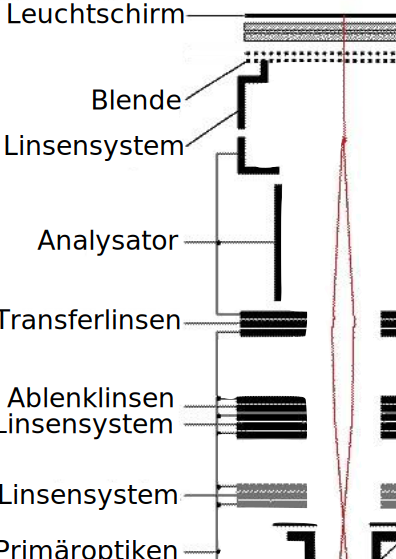
\includegraphics[width=0.7\textwidth]{./content/PEEM_schemaneu.jpg}
            \caption{Exemplarischer Aufbau eines Momentum Microskope. Aus \cite{KUCH}.}
            \label{fig:MM}
        \end{figure}
        Ein exemplarischer Aufbau ist in Abbildung \ref{fig:MM} zu sehen.
        Die durch die Photonen angeregten Elektronen werden durch ein starkes elektrisches Feld von einigen \si{\kilo\volt} von der Probe zum Analysator hin beschleunigt.
        Das Extractorfeld kann bis auf \SI{29}{\kilo\volt} erhöht werden, wird standardmäßig aber auf \SI{10}{\kilo\volt} festgesetzt
        Durch diese große Spannung zwischen Probe und Extraktor ist es möglich ein ein großen Sichtbereich im Impulsraum abzudecken.
        Dies ist nötig, da durch den streifenden Einfall der Photonen und der Abberation der elektrostatischen Linsen nur einen kleinen Akzeptanzwinkel zur Verfügung stehen würde. \textbf{QUELLE}
        Wichtig bei der Kathoden Linse ist, dass das Feld zwischen Probe und Linse sehr homogen ist, damit der Austrittswinkel erhalten bleibt.
        Anschließend werden die Elektronen durch elektrostatische Linsen fokusiert und durch die einzelnen Blenden geleitet.
        Sie sind so konzipiert, dass die Bildebene und die hintere Brennebene immer an der selben Position, der Blenden bleiben.
        Mit Hilfe von Kontrastblenden kann dann eine Auflößung von einigen \si{\nano\meter} erreicht werden. \textbf{QUELLE}.
        Hierbei gibt es an zwei verschiedenen Stellen Blenden, je nach dem ob im Realraum oder im Impulsraum ein Bild aufgenommen werden soll.
        Damit der Spot auch immer im Zentrum der Blenden liegt gibt es im Linsensystem noch elektrostatische Verschiebungslinsen, welche den Strahl ablenken.
        Nach den Blenden folgt ein weiters Linsensystem aus elektrostatischen Linsen, welche das Bild auf den Ausgang des Linsensystems fokussieren.
        Hier befinden sich zwei magnetische Verschiebungslinsen um Drift zu korrigieren.
        Im Anschluss gehen die Elektronen in ein Transferlinsensystem über, welches dafür sorgt, dass ein einszueins Abbild auf die Eingagnsblende das Analysators trifft.
        Die Eingagnsblende kann in ihrer Größe varriert werden, sodass nur ein Teil der Elektronen in den Analysator eintreten.
        Je kleiner die Blende gewählt wird, desto besser ist die Energieauflösung aber so kleiner die Gesamtintensität.
        Im Analysator selbst unterliegen die Elektronen der energieabhängigen Dispersion im elektrischen Feld. 
        Nur Elektronen mit der passenden Energie verlassen den Analysator durch die Ausgangsblende.
        Nach dem Detektor gibt es eine weiter Linseneinheit, welche zusammen mit einer Blende das gewünschte energieaufgelöst Bild auswählt und es auf die Detektorgröße aufweitet.
        Anschließend durchlaufen die Elektronen eine Mikrokanalplate (eine Art Elektronenvervielfacher) und prallen auf den Phosphorschirm, der an den entsprechenden Stellen aufleuchtet.
        Durch die Kamera wird diese Leuchten regestriert und das räumliche oder rekrusives Bild kann rekostruiert werden \cite{SPECS-MM}.

        \subsection{Impulsraum Aufnahmen}
        Bei der Aufnahme im Impulsraum wird bei der gesamten Abbildungsoptik der Austrittswinkel erhalten.
        Das verwendete Mikroskop kann einen Austrittswinkel von biszu $\pm\SI{90}{\degree}$ erfassen für eine Energie kleiner als \SI{50}{\electronvolt} \cite[page=21]{SPECS-MM}.
        Für größere kinetische Energien wird das Sichtfeld auf $\pm\SI{3.6}{\angstrom}$ beschränkt.
        Dabei spielt es keine Rolle wo auf der Probe die Elektronen emittiert werden.

        Um ein Bild im Impulsraum aufzunehmen wird die Blende im der Bildebene eingefahren, die so genannte Feldblende (\textit{field aperture}).
        Durch die Blende wird ein Ausschnitt auf der Probe ausgwählt, von der die emittierten Elektronen erfasst werden.
        Bei einem Blendendurchmesser von \SI{20}{\micro\meter} und der Standard-Vergrößerung von \num{5} ist der ausgewählt Bereich etwa \SI{4}{\micro\meter} groß.

        \subsection{realraum Aufnahmen}
        Es ist ferner möglich Bilder im Realraum aufzunehmen. 
        Dabei können sehr kleine Spots von \SIrange[range-pharse=' bis ']{50}{200}{\micro\meter} ausgewählt werden.
        Das Bild wird dann bei festen Energiefilter-Einstellungen aufgenommen.

        Um den Kontrast im Bild zu erhöhen werden nur Elektronen mit einem bestimmten Austrittswinkel für die Erstellung des Bildes erfasst.
        Dies geschieht durch Einsetzen einer Blende in dem hinteren Brennpunkt, die Kontrastblende (\textit{contrast aperture}).



        \begin{figure}
            \centering
            \includegraphics[width=0.7\textwidth]{./content/Real_k.PNG}
            \caption{Die verschiedenen Konfiguration der Blenden um zwischen Realraum Bild und Impulsraum Bild umzuschalten. Aus \cite{Focus}.}
            \label{fig:real_k}
        \end{figure}
        Für den Impulsraum ist dies in Abbildung \ref{fig:real_k}\,a und für den Realraum in Abbildung \ref{fig:real_k}\,b dargestellt.
        Um ein Bild im Realraum zu erhalten muss die Blende im Brennpunkt eingesetzt sein, auf dem Eintrittsspalt des Energyanalysators wird dann das Bild der Oberfläche projeziert.
        Wird hingegen in der ersten Bildebene die Blende eingesetzt so wird auf dem Eintrittsspalt das Beugungsbild abgebildet. 
        Die restlichen Linsen, Stigmatoren und Ablenker sind dafür da, dass Bild zu zentrieren und Abberation auszugleichen.

        Als Energiealysator kommt ein hemisphärischer Analysator zum Einsatz, für gepulste Photonenquellen würde sich auch ein \textit{Time of flight - TOF} (Flugzeit) Analysator eignen.
        Bei dem hemisphärischer Analysator werden die Elektronen zwischen zwei Halbkugeln durch ein statisches elektrisch Feld auf eine Kreisbahn gezwungne.
        Dabei ist das Feld so gewählt, dass nur die mit der richtigen kinetischen Energie eintretenden Elektronen auch auf den Austrittsspalt abgebildet werden.
        Bei einem TOF Analysators wird die kinetische Energie aus der Flugzeit der Elektronen bestimmt, weswegen es nur für gepulste Photonenquellen möglich ist.

        Nach dem Energiealysator gibt es nochmal ein paar Optiken, die das Bild auf den Detektor abbilden.
        Bei dem Detektor handelt es sich um eine CMOS Kamera die das Bild der auf den Leuchtschirm auftreffenden Elektronen aufnimmt.
        Der Vorteil der CMOS (\textit{Complemantary metal-oxid-semiconductor}) Kamera Technik gegnüber der klassischen CCD (\textit{Charge Coupled Device}) Kamera Technik ist, dass erlaubt es wahre Pulszählraten zu erfassen 
        Dabei wird ein einzelnes Bild in nur wenigen Millisekunden erfasst, dies ist durch die Kombination von Kamera und Grafigprozessor möglich.
        Die CCD Detektoren sind ein Standard bei ARPES Messungen, sie integrieren die analoge Photonenintensitäten oder einzelne Lichtblize werden aufgezeichnet.
        Einer der Nachteile ist die geringe Abtastrate auf Grund der hohen Erholungszeit.

        \cite{CMOS}.

      
        \begin{figure}
            \centering
            \includegraphics[width=0.7\textwidth]{./content/MM.png}
            \caption{Der für die durchgeführten Experimente verwendete Aufbau.}
            \label{fig:aufbau}
        \end{figure}
        Der gesamte Aufbau aus dem PEEM und der Präperationskammer ist in Abbildung \ref{fig:aufbau} zu finden.

        \begin{itemize}
            \item Erweiterung auf Spinaufgelöst möglich
            \item TOF
            \item Zeitaufgelöst
            \item Real und Impulsraum
        \end{itemize}

    \section{Molekül Orbital Tomographie}
        Die Molekühle Orbital Tomographie vereinigt nun die Vorteile des Momentum Mikroskopes mit der Theorie der Dichtefunktionaltheorie (DFT) um Molekühlorbitale zu identifizieren.
        \begin{itemize}
            \item Vereinigung von Experiment und Theorie
            \item MM
        \end{itemize}


\chapter{Ergebnisse}
\section{Vorbereitung und Präperation}
    \begin{itemize}
        \item Sputtern und annealen
        \item Gold
        \item NiO
        \item Moleküle
        \item LEED-Bilder
    \end{itemize}

\section{Datenformat und Bearbeitung}
    \begin{itemize}
        \item 3D Cubes
        \item BE 
        \item px to k
        \item symmetrisieren
    \end{itemize}

\section{Integrierte Spektren}
    \begin{itemize}
        \item Sieht Features später Zuordnung
        \item Ändert sich was
    \end{itemize}

\section{Bandstruktur}
    \begin{itemize}
        \item Bandstruktur von Gold
        \item Bandstruktur NiO? Spin?
        \item Bandstruktur mit Molekülen - Oberflächenzustände? Extra Features
    \end{itemize}

\section{Maps}
    \begin{itemize}
        \item Maps selbst die sich zuordnen lassen
        \item Aus den LP bestimmte zuordnung möglich?
    \end{itemize}
% \input{content/04_Ergebnisse_alt.tex}
\chapter{Zusammenfassung und Ausblick}
    Zusammenfassend lässt sich sagen, dass sich die Präperation von wohldefinierten dünnen Übergangsmetalloxiden als recht schwierig erweist und genauere Untersuchungen benötigt werden.
    Besonders hinsichtlich von Kontaminationen und Stochimetrie, sowie der Oberflächenbeschaffenheit sind Verbesserungen von nöten.
    Bevor weitere Untersuchung der Wechselwirkung mit Molekülen durchgeührt werden, sollten zunächste die Substrate vollständig charakterisiert und reproduzierbar präperiert werden.
    Denn wie bei ferromagnetisch Systemen sind die Eigenschaften des zugrundeliegenden Systems entscheidend für den Spintransport~\cite{IF_16}.

    Nickeloxidfilme lassen sich ohne große Probleme durch aufdampfen in einem Sauerstoffdruck erzielen.
    Hierbei wird die polare und instabile (111)-Oberfläche durch eine \ce{OH-}-Kontamination stabilisiert.
    Beim Aufdampfen von Eisen in einer Sauerstoffatmosphäre kommt es zunächst zu einer gemischten Eisenoxidphase.
    Durch dan Einfluss des ioneninduzierten Zerstäuben führt dies zur Phase des \ce{FeO}.
    
    Für das Nickeloxis zeigt sich für unterschiedliche Schichtdicken verschiedenen Energienieveauanpassungen der Molekülorbitale.
    So wurde für das Nickeloxidfilm ebenfalls gezeigt, dass eine zu reaktive Oberfläche die Selbstanordnen behindern kann.
    Wohin die weniger reaktive Oberfläche des Wüstit die Selbstanordnen unterstütz, was sich mittels der Molekülorbitaltomographie bestätigen lässt.
    Ferner wird trotz der isolierenden Eigenschaft einen Ladungsaustausch mit den Molekülen begünstigt und das LUMO wird besetzt.

    weitergehende Untersuchungen im Bereich von Spin aufgelöste Messungen wären denkbar um den Effekt des Antiferromagneten und den Einfluss auf die Molekülbesetzung zu interpretieren.
    So eignet sich die Spin aufgelöste Molekülorbitaltomographie zur charakterisieren der Molekülorbitale.
    Mit der Messung von Röntgenabsorptionsspektren für verschiedene Polarisationen kann die Ausrichtung der Moleküle und die magnetischen Eigenschaften der einzelnen Beteiligten bestimmt werden.
    Unterschiedliche Schichtdicken und Austrittsarbeiten durch die Sauerstoffkonzentration sollten Beachtung finden um die Energieniveauanpassung weiter gehend zu otimiereen~\cite{IF_8}.
    Auch die Absorptionsstärke lässt sich hierdurch, sowie der Wahl der Oberflächenorientierung beeinflussen.


\appendix
% Hier beginnt der Anhang, nummeriert in lateinischen Buchstaben
% \chapter{Ein Anhangskapitel}

Hier könnte ein Anhang stehen, falls Sie z.\,B.\ Code, Konstruktionszeichnungen oder Ähnliches mit in die Arbeit bringen wollen.
Im Normalfall stehen jedoch alle Ihre Resultate im Hauptteil der Bachelorarbeit und ein Anhang ist überflüssig.

\section{Einkristalloberflächen}
        Die geordneten Strukturen eines Einkristalls kommen durch die Wechselwirkung der Elektronen zwischen den einzelnen Atomen.
        So ergibt sich eine periodische Anordnung der Atome im thermischen Gleichgewicht.
        Dabei sind die Atome nicht komplett starr an ihre Plätze gebunden, sondern führen kleine Schwingungen um diesen aus.
        Mit der Temperatur sinkt auch die Auslenkung.
        Dieses Wechselspiel der strukturellen Ordnung findet sich auch in der elektronischen Struktur wieder.
                
        Wird ein Einkristall entlang einer Kristalleben durchschnitten so ergibt sich eine Oberfläche.
        Die Ebene erhält den Namen der Indizes des auf ihr senkrecht stehenden Gittervektors $r_{hkl}$, also $(hkl)$.
        Als Oberfläche werden die oberen Atomlagen definiert, die sich in der geometrischen und/oder chemischen Art von der des Volumens unterscheiden~\cite{Fauster}.
        Aufgrund der nun fehlenden Bindungen nach oben ergeben sich neue elektronische und geometrische Eigenschaften.
        So kann es zu lateralen und transversalen Verschiebungen gegenüber der volumenartigen Struktur, so genannte Rekonstruktionen und Relaxation kommen.
        Dabei ordnen sich die Atome um, um damit einen energetisch günstigeren Zustand zu erhalten.
    
        Wie im Volumenkristall kann die Oberfläche durch eins von fünf Bravais-Gittern beschrieben werden, wobei auf jedem Gitterpunkt eine atomare Basis gesetzt wird.
        Die Punkte dieses zweidimesionalen Gitters lassen sich durch den Gittervektor
        \begin{equation}
            \vec{r}_{nm} = n \vec{a}_1 + m \vec{a}_2
            \label{eqn:Gittervek}
        \end{equation}
        mit $n,m \in \mathbb{Z}$ und den Vektoren der Einheitszelle $\vec{a}_1, \vec{a}_2$ beschreiben.
        Geimeinsam legt das Bravais-Gitter und die atomare Basis die Symmetrien der Oberfläche fest.
    
        Durch die Anlagerung von Adsorbaten können Symmetrien der Oberfläche verloren gehen.
        Die Struktur der Adsorbate relativ zur Oberfläche wird Überstruktur genannt.
        Durch den meist größeren Abstand der Adsorbate untereinander als der Basen des Substrates ergibt sich auch eine größere Einheitszelle.
        Beim Schneiden der Einkristalle um eine Oberfläche zu erhalten können sich unter anderem auch Stufen ausbilden.
        Vermehrt treten diese Stufen bei hochindizierten Oberflächen auf, wobei einzelne Terrassen dann eine niedrigindizierte Oberfläche darstellen~\cite{Fauster}.
        Diese Stufen oder auch Defekte in der Oberfläche bilden Keimzellen für Anlagerung von Adsorbaten.
        Um die Überstruktur des Adsorbate zu beschreiben wird die von ihnen aufgespannte Einheitszelle aus den Gittervektoren des Substrats rekosntruiert.
        Die Gittervektoren des Übergitters $\vec{b}_1, \vec{b}_2$ lassen sich dann als Matrixschreibweise darstellen.
        Damit ergibt sich auch die Überstrukturmatrix $C$ mit 
        \begin{equation}
            \begin{pmatrix}
                \vec{b}_1 \\
                \vec{b}_2 \\
            \end{pmatrix}
            = 
            \begin{pmatrix}
                C_{11} & C_{12} \\
                C_{21} & C_{22} \\
            \end{pmatrix}
            \begin{pmatrix}
                \vec{a}_1 \\
                \vec{a}_2 \\
            \end{pmatrix}.
        \end{equation}
        Relative Verschiebungen zum Substrat bleiben dabei ohne Beachtung, es zeigt nur die Periodizität der Struktur an.
        Ferner kann es zur Aubildung verschiedener Domänen kommen, besonders dann, wenn die Symmetrie des Übergitters kleiner als die des Substrates ist~\cite{Fauster}.
        Einzelne Domänen weisen Symmetrie äquivalente Anordnungen auf, häufug handelt es sich nur umgedrehte Einheitszellen.
        Nicht nur Adsorbatebedeckungen lassen sich durch diese Notation beschreiben, auch die Rekonstruktion der Oberfläche.
        Hierbei sind es keine Adsorbatatome, sondern die Oberflächenatome selbst, die eine neue Struktur ausbilden.
        Die Relaxation, welche die Änderung im Lagenabstand beschreibt kann hingegen nicht durch dies Notation beschrieben werden.
        Sie ist ebenso wie die Rekonstruktion vom Material, der Kristallstruktur und der Oberflächenorientierung abhängig.
        Einige Rekonstruktionen und Relaxation hängen auch vom Präperationsprozess ab, wenn die Oberfläche selbst metastabil ist.
    
        Wie bereits erwähnt hängen geometrische und elektronische Struktur stark zusammen.
        Sodass sich an Oberflächen durch die fehlenden Bindungen die elektronische Struktur verändern kann.
        Die quantenmechanische Beschreibung der Elektronen erlaubt es auch die elektronischen Zustände der Oberfläche durch Quantenzahlen auszudrücken.
        Hier ist $\vec{k}_{||}$ der Wellenzahlvektor der Oberfläche die Ausschlag gebende Größe um die Oberflächenbandstruktur $E(\vec{k}_{||})$ zu beschreiben.
        Ganz besondere Beachtung erhalten die Zustände nahe der Fermikante $E_\text{F}$ die für leitenden Eigenschaften verantwortlich sind.
        Erhaltene Oberflächenbandstruktur kann von der der Volumenbandstruktur abweichen.
        Dies führt zum Teil zu Oberflächenzuständen, die unterscheiden sich energetisch von denen im Volumenkristall und können somit nur in dessen Bandlücke auftreten.
    
        % Ein wichtiger Ansatz für die periodische Struktur der Oberfläche und dessen elektronischen Zustände ist das Bloch Theorem.
        % Die Oberfläche entspricht einer Anordung äquivalenter Punkte welche durch den Gittervektor aus \autoref{eqn:Gittervek} ineinander überführt werden können

        \subsection{Eisen (100) Oberfläche}
            \begin{itemize}
                \item WKF
                \item Symmetrie - p4mm
                \item Gitterkonstante ist $a = \SI{2.862}{\angstrom}$~\cite{springer_database}
                \item bcc Struktur
            \end{itemize}
        
        \subsection{Gold (111) Oberfläche}
            Gold gehört zu den Edelmetallen und kristallisiert in der flächenzentrierten Struktur mit einer Gitterkonstanten von \SI{4.08}{\angstrom}~\cite{Marx}.
            Es ist besonders leitfähig, stabil und wenig reaktiv, dennoch rekosntruiert die Oberfläche in einer Fischgräten-Struktur ($\num{22} \times \sqrt{\num{3}}$)~\cite{5A_3}.
            Die Austrittsarbeit der (111)-Oberfläche wurde dabei auf \SI{5.46}{\electronvolt} bestimmt~\cite{5A_4}.
            Ebenfalls bildet sich auch ein sehr präsenter Oberflächenzustand aus.
            
            Auf Grund der sehr ähnlichen Gitterkonstante zu der des Nickeloxids von nur etwa \SI{2}{\percent} eignet es sich besonders gut als Substrat \cite{NiO_36}.
            \begin{itemize}
                \item Ebenenabstand in Au(111) $d_0 = \SI{2.35}{\angstrom}$.\textbf{\cite{5A_1}}
            \end{itemize}

            Bereits bekannt ist, dass sich auf diesem Substrat das Pentacene anordnet~\cite{5A_1, 5A_3}.
            Die lange Molekülachse liegt dabei parallel zu den Reihen der Goldatome, mit den äußeren Ringen und somit die $\pi$-Orbitale direkt oberhalb eines Goldatoms.
            Diese Positionierung lässt auf eine starke Substrat-Molekül-Interaktion schließen~\cite{5A_3}.
            Bei der Wechselwirkung dieser handelt es sich um Physisorption, was damit auch die Adsorbate-Adsorbat-Wechselwirkung zur Formung der Einheitszelle dominieren lässt~\cite{5A_4}.
            Ferner liegen in einer Monolage flach auf der Oberfläche und einzelne Reihen sind durch eine Reihe Goldatome separiert.
            Allerdings wächst der Pentacenefilm nicht epitaxtisch, sondern in Form von Inseln mit unterschiedlichen Einheitszellen~\cite{5A_3}.

            \begin{figure}
                \centering
                \includegraphics[width=0.5\textwidth]{Au+5A/EDC_Au_5A_mod.png}
                \caption{Die integrierten Spektren für reines Gold, Gold mit einer Monolage Pentacene und deren Differenz.}
                \label{fig:EDC_Au+5A}
            \end{figure}
            Das Goldsubstrat eignet sich ebenfalls zur Kalibrierung der Monolage von Pentacene, da bereits bekannt ist, dass sich diese flach auf der Oberfläche ordnet \cite{5A_1}.
            Bei der Wechselwirkung mit dem Substrat handelt es sich um die Physisorption durch einen Substrat-Molekülabstand von \SI{3.28}{\angstrom} \cite{5A_1}.
            % Es ergibt sich so das LEED-Bild in \autoref{fig:LEED_Au+5A}, was auch die bekannte \textbf{Überstruktur} (5A_1, 5A_5) aufweist.
            Schaut man sich das winkelintegrierte Spektrum im Bereich der Valenzzustände in \autoref{fig:EDC_Au+5A} an, so sind auch deutlich Elemente zu erkennen, die durch die Moleküle hervorgerufen werden.
            Die senkrechten Linien stellen die Punkte da, an denen Bilder mit höherer Statistik aufgenommen wurden und die später zur Molekülorbitalanalyse herangezogen werden.
    
            \begin{figure}
                \centering
                \begin{subfigure}[t]{0.48\textwidth}
                    \centering
                    \includegraphics[height=4cm]{Au+5A/MOT_Au_5A_exp_1.png}
                    \subcaption{Gemmesen, symmetrisiertes Bild bei einer Bindungsenergie von \SI{0.8}{\electronvolt}.}
                    \label{fig:MOT_Au+5A_exp_1}
                \end{subfigure}
                \begin{subfigure}[t]{0.48\textwidth}
                    \centering
                    \includegraphics[height=4cm]{Au+5A/HOMO_all_CT}
                    \subcaption{Das theoretisch erwartete HOMO.}
                    \label{fig:MOT_Au+5A_theo_1}
                \end{subfigure}
                \centering
                \begin{subfigure}[t]{0.48\textwidth}
                    \centering
                    \includegraphics[height=4cm]{Au+5A/MOT_Au_5A_exp_2.png}
                    \subcaption{Gemmesen, symmetrisiertes Bild bei einer Bindungsenergie von \SI{1.85}{\electronvolt}.}
                    \label{fig:MOT_Au+5A_exp_2}
                \end{subfigure}
                \begin{subfigure}[t]{0.48\textwidth}
                    \centering
                    \includegraphics[height=4cm]{Au+5A/HOMO1_all_CT}
                    \subcaption{Theorie Oribtale mit Symmetrisierung des HOMO-1.}
                    \label{fig:MOT_Au+5A_theo_2}
                \end{subfigure}
                \begin{subfigure}[t]{0.48\textwidth}
                    \centering
                    \includegraphics[height=4cm]{Au+5A/MOT_Au_5A_exp_3.png}
                    \subcaption{Gemmesen, symmetrisiertes Bild bei einer Bindungsenergie von \SI{2.65}{\electronvolt}.}
                    \label{fig:MOT_Au+5A_exp_3}
                \end{subfigure}
                \begin{subfigure}[t]{0.48\textwidth}
                    \centering
                    \includegraphics[height=4cm]{Au+5A/HOMO2_all_CT}
                    \subcaption{Berechnetes Theoriebild zum HOMO-2.}
                    \label{fig:MOT_Au+5A_theo_3}
                \end{subfigure}
                \caption{Zuordnung eines Bildes zu einem der Molekülorbitale. Theorie Oribtale mit Symmetrisierung zweimal um 120 Grad gedreht und zum Ursprungsbild addiert.}
                \label{fig:MOT_Au+5A}
            \end{figure}
            Winkelaufgelöste Bilder bei den entsprechenden Energien zeigen auch zusätzliche Merkmale im Bezug zum reinen Gold.
            Gemeinsam mit theoretischen Berechnungen aus der Dichtefunktionaltheorie lassen sich diese dann entsprechenden Molekülorbitalen zuordnen.
            Dies ist für einige Energien und Orbitale in \autoref{fig:MOT_Au+5A} geschehen.
            Dabei wurden die gemessenen wie auch berechneten Bilder entsprechend der Geometrie aus dem Beugungsbild \autoref{fig:LEED_Au+5A} jeweils um \SI{120}{\degree} gedreht und aufsummiert.
    
            Eine Zuordnung einer der markanten Elemente zu einem zuvor unbestzten Orbital, dem LUMO ist nicht zu erkennen.
            Es scheint also so als würden keine Elektronen zwischen Substrat und Molekül ausgetauscht werden. 
            Dies lässt sich auch aus der Literatur erkennen, dass sich bei den Anornung von Pentacene auf Gold um den Prozess der Physisorption handelt~\cite{5A_4}.
            Abwesenheit des LUMOs in den Spektren und Bildern muss aber nicht zwangsläufig auf die Physisorption hindeuten.
            So ist Pentacene auf Kupfer (111) chemisch adsorbiert und zeigt dennoch keine Anzeichen der Besetzung des LUMO~\cite{koch_adsorption-induced_2008}.

\backmatter
\printbibliography


\cleardoublepage
\includepdf[fitpaper=true]{content/Eidesstattliche_Versicherung.pdf}
% \input{content/eid_versicherung.tex}
\end{document}
